\chapter{Literature Review}\label{chapter:literature_review}

\section{Message Passing Paradigm}
\label{sec:messagePassing}
  Message passing is sending a message from one process, component or actor to another. Message passing is the loosest form of coupling. The components of a system are not dependent on each other; instead they use a public interface to exchange parameterless messages\cite{joecelko}. Hence, systems that implement the message passing paradigm are easily scalable and efficient. Such systems are easy to replicate and make fault-tolerant.
~\cite{Armstrong:2010:ERL:1810891.1810910}.

  Systems which communicate solely by message passing do not have a shared state. Such systems can be easily divided into isolated components. This makes the overall architecture easy to understand and simplifies isolation of problems within the system~\cite{Armstrong:2010:ERL:1810891.1810910}.

  Message passing can be synchronous or asynchronous. Synchronous message passing is a communication between two components where the sender blocks until it gets a response from the receiver. Whereas, in asynchronous message passing, the sender simply sends a message and continues to do other tasks. The receiver does not have to be ready to accept the message when the sender sends it~\cite{agha}. Thus, asynchronous message passing is non-blocking in nature.

  When a message is received by a recipient, the recipient chooses further processing based on the pattern or content of the message.

\section{Actor Programming Model}
\label{sec:actorProgramming}
  The actor model is a programming paradigm designed for concurrent computation. The concept of an actor was originally introduced by Carl Hewitt\cite{hewitt}. He, along with Agha\cite{agha} have been involved in development of the actor theory as well as its implementation.

  An actor is a fundamental unit of computation. It is neither an operating system process nor a thread, but a lightweight process~\cite{hewittVideo}. %process or thread ? lookup
  It embodies three essential things:
\begin{itemize}
  \item Processing
  \item Storage
  \item Communication
\end{itemize}
  Actors have addresses and there is a many-to-many relationship between actors and addresses.

  Actors communicate with each other in a non-blocking way by asynchronous message passing, which removes the need for explicit locks. An actor can send messages to actors in the same actor system or another actor system. An actor can also send messages to itself, which is how recursion is achieved. An actor can send a message to a target actor only if it has its address. Agha~(\cite{agha}, p35) lists three ways in which an actor, upon accepting a message, can know the address of the target actor:
  \begin{itemize}
    \item the target was known to the actor before it accepted the message
    \item the target became known when the message was accepted because its address was contained in the message
    \item the target is a new actor created as a result of accepting the message
  \end{itemize}

  To buffer incoming messages, each actor has a mailbox. A mailbox is a queue of messages that have been sent by other actors or processes and not yet consumed, where the mailbox is also an actor. According to Hewitt, the order in which messages are delivered is non-deterministic~\cite{hewittVideo}.

After receiving a message, an actor may perform the following actions~\cite{hewitt}:
\begin{itemize}
  \item Create other actors
  \item Send messages to itself, other known actors or reply to the actor that sent the message
  \item Designate how it is going to handle the next message, i.e. Specify a replacement behavior
\end{itemize}

  Actors do not have a shared mutable state. All mutable state is private to the actor and all shared state is immutable. Actors communicate with each other by asynchronous message passing, where messages are immutable. Each actor processes only one message at a time, and unless it is a broadcast message, a message is not processed multiple times.

  An actor exists in a group of actors working together in a certain hierarchy called an \emph{actor system}.

  In the actor model, concurrency is inherent because of the way it is designed. Also, there is no guarantee that messages sent to an actor arrive sequentially~\cite{hewittVideo}. Nevertheless, the Akka framework~[\autoref{sec:akka}] guarantees the order of delivery of messages between two actors, provided that there are no intermediary actors~[\autoref{subsec:akkaMessagePassing}].

  Several programming languages like Act 1, Act 2, Act 3 and Acttalk were created when actors were newly introduced by Hewitt and Agha~\cite{agha, hewitt}.

\subsection{Error Handling in the Actor Model}
Error handling in the actor model is based on the idea of embracing failure. The idea of embracing failure is also known as the “let it crash” philosophy~[\autoref{subsec:letItCrash}]. As actors do not have shared state, this allows individual actors to fail without causing disruption in the system. Since an actor in an actor system is typically organized in a hierarchy, the actor which created a child actor can be used for supervising it. The idea of supervision in a hierarchical actor system helps to make the actor system fault tolerant~\cite{Erb2012}. When an actor throws an exception the supervisor can respond to the exception in different ways. In Akka~[\autoref{sec:akka}], the supervising actor usually reacts by either simply ignoring the exception and letting the actor continue, by restarting the actor or by escalating the error to its supervisor.

  The “let it crash” philosophy is a non-defensive programming style, which is implemented in Erlang~[\autoref{sec:erlang}] and Akka.

\subsection{Differences from Thread-based Programming Model}
\subsubsection{Thread-based Concurrency}
  \label{subsec:thread}
  In thread-based programming languages, the control flow of a program is divided into several threads for concurrency. When two or more threads have shared memory, concurrent modification and access of data may result in undesired behavior of the system, known as a ‘race condition’. To prevent this type of situation, thread-based programming languages use locks. Locks restrict more than one thread to execute a section of program code~\cite{ambientTalk} concurrently.

  Generally thread-based programming models are easy to understand and implement. But the resulting program behavior is difficult to comprehend because of implicit context switches and release of locks, which may lead to a deadlock situation~\cite{ambientTalk}.

\subsubsection{Actors Based Concurrency}
\label{subsec:actorConcurrency}
  Concurrency in actor based programming languages is inherent because of asynchronous message-passing, pipelining, and dynamic creation of actors. Concurrency in actors through pipelining is only constrained by logical limits and available hardware resources~\cite{agha}. Actors may carry out their activities in parallel, as each actor resides in a completely separate space and interacts only via messages.

  Actor based programming liberates programmers from delving into coding details about parallelism and threads~\cite{agha}.

  ‘Race conditions’, as discussed in \autoref{subsec:thread}, do not arise in actor based programming, as actors do not have shared state and do not need locks.

\subsection{Scaling Actor Based Systems}
  As actor based systems are highly concurrent~[\autoref{subsec:actorConcurrency}], it is easy to scale them from a single core system to a cluster of multi-core systems, distributed across the globe. An ideal case for scaling would be to let a new node join a cluster and dynamically expand an actor system with zero downtime. The actors themselves do not need to know the physical location of other actors as they simply exchange messages based on logical addresses. This makes them easy to scale up by adding more actors to the same machine and scale out by adding more nodes to a cluster.

\section{Erlang}
\label{sec:erlang}
  Erlang is the first popular programming language based on the actor model~\cite{vinoski}. It was developed by Joe Armstrong in 1986 at the Ericsson Computer Science Laboratory and was made open-source in 1998. It was chiefly used in telephony applications as it was built to solve the problems of availability and scalability that existed in such applications~\cite{armstrong}.

  Erlang ‘processes,’ which are essentially user-space threads rather than Unix processes or kernel threads, communicate only via message passing.~\cite{armstrong}

  Erlang was designed for writing applications that require high availability~\cite{armstrong}. It uses concurrent processes, which have no shared memory and communicate only via asynchronous message passing. This idea is similar to the actor model proposed by Agha and Hewitt~[\autoref{sec:actorProgramming}]. Thus, programs written in Erlang are concurrent, distributed, fault tolerant and thread safe. Concurrency is built into the language~\cite{Armstrong:2010:ERL:1810891.1810910}.

  When an application developed in Erlang is deployed in a multi-core computer, it automatically takes advantage of those cores. So, programmers do not have to worry about threads~\cite{Armstrong:2010:ERL:1810891.1810910}. In Erlang, new changes in an application can be added to a system without taking it offline. This improves availability of the whole system, simplifying construction of software for implementing non-stop systems~\cite{armstrong}.

  Error handling in Erlang is different from most other programming languages. Error handling is based on a “let it crash” philosophy~[\autoref{subsec:letItCrash}] which is a non-defensive style of programming~\cite{armstrong, Armstrong:2010:ERL:1810891.1810910}.

\subsection{“Let it Crash” Philosophy}
\label{subsec:letItCrash}
  The core idea of the “Let it Crash” philosophy is to let failing processes crash, having supervising processes detect and fix the crashes~\cite{Armstrong:2010:ERL:1810891.1810910}. Error handling in Erlang and the supervision strategy in Akka~\autoref{sec:akka} are based on this principle.

   This idea is in sharp contrast to other programming languages, where programmers implement exception handlers and prevent a process from being terminated.

  Proponents of the “let it crash” philosophy argue that it leads to more clear and compact code~\cite{Armstrong:2010:ERL:1810891.1810910}.

\section{Scala Actors}
\label{sec:scala}
Scala is a statically typed programming language which integrates functional as well as object-oriented programming~\cite{Odersky}. Scala has its own library for actor programming. In Scala, templates for actors with user-defined behavior are normal class definitions which extend the predefined Actor class.

  The Scala actors library provides a concurrent programming model based on actors~[\autoref{sec:actorProgramming}]. Actors in scala are fully interoperable with ordinary virtual machine threads~\cite{Haller}. Scala actors are lightweight and support approximately 240 times more actors to run simultaneously compared to virtual machine threads~\cite{Haller}.

  Both synchronous and asynchronous message passing may be used in Scala actors. Synchronous message passing is implemented by exchanging several asynchronous messages. Actors in Scala can also communicate using ‘futures’. When a future is used requests are handled asynchronously and the sender immediately gets a representation of the future which allows the sender to wait for the reply~\cite{scalaActors}.

  The Scala actors library is now deprecated and will be removed in future Scala releases\footnote{Scala actors are deprecated in version 2.10~\cite{scalaActorsAPI}}. The deprecation is in favor of the use of Akka actors~[\autoref{sec:akka}].

\section{Akka Toolkit}
\label{sec:akka}
Akka is a toolkit and runtime for building highly concurrent, distributed and resilient message-driven applications on the JVM (Java Virtual Machine)~\cite{akkaHome}. Akka uses lightweight actors for concurrency. Actors in Akka are based on Hewitt and Agha's model~\cite{agha, hewitt}. Akka provides a well defined API for developers to create large concurrent systems, which allows for easily scaling out.
  Akka is available for Scala as well as Java.

  \subsection{Actor Model in Akka}
  Akka actors are objects which encapsulate state and behavior,  communicating only by message passing, similar to Hewitt and Agha's model~[\autoref{sec:actorProgramming}]. As Akka actors are objects, they enforce a stringent form of object-oriented programming~\cite{akkaActorSystem}.

  The ‘ActorRef’ in Akka represents an actor and holds a reference to an actor. Its purpose is to facilitate message sending to the actor it references. An actor can also refer to itself using \emph{self} \cite{akkaJavaDoc}.

  \autoref{lst:akkaHelloWorld}~\footnote{Source: \fullcite{akkaHome}} is an example of how actor programming in Akka is realized. In this example, the ‘GreetingActor’ which extends ‘UntypedActor’ must implement the \emph{onReceive()} method. The \emph{onReceive()} method is invoked for each message received by this actor. After receiving a message, the actor performs pattern matching to decide which code to execute. If the message is a type of ‘Greeting’ object, it is concatenated with the string “Hello” otherwise, it is simply ignored.

\begin{lstlisting}[caption=A simple example of actor programming in Akka~\cite{akkaHome}, label=lst:akkaHelloWorld]
public class Greeting implements Serializable {
  public final String who;
  public Greeting(String who) { this.who = who; }
}

public class GreetingActor extends UntypedActor {
  LoggingAdapter log = Logging.getLogger(getContext().system(), this);

  public void onReceive(Object message) throws Exception {
    if (message instanceof Greeting)
      log.info("Hello " + ((Greeting) message).who);
    }
}

ActorSystem system = ActorSystem.create("MySystem");
ActorRef greeter = system.actorOf(Props.create(GreetingActor.class), "greeter");
greeter.tell(new Greeting("Charlie Parker"), ActorRef.noSender());
\end{lstlisting}


  \subsection{Actor System}
  \label{subsec:actorSystem}
    An actor system in Akka arranges actors in a hierarchy. The hierarchy of actors are formed by an actor creating child actors to handle certain tasks. An actor not only creates and assigns tasks to child actors but also supervises them~[\autoref{subsec:supervisionMonitoring}]. Thus it is implicit that there can be only one supervisor of an actor.

  By splitting up tasks, they become clear and structured. Furthermore, the resulting actors become simplified and specialized in terms of which messages they should process and how they should react. It also becomes easier to handle failures. If an actor cannot cope with a failure, it is escalated up the hierarchy to its supervisor. The escalation is repeated by each parent actor in the hierarchy until it reaches an actor that can handle the failure~\cite{akkaJavaDoc}.

  An actor instance in Akka takes up roughly 300 bytes of memory, allowing the spawning of millions of them in one actor system. Akka is able to manage the order of message processing even in large systems with millions of actors~\cite{akkaJavaDoc}.

  An example of the arrangement of actors in a hierarchy is shown in \autoref{fig:actorSystem}. The ‘{$\backslash$}’ is known as a “root guardian” and \emph{$\backslash$user} is known as a “user guradian”. Any actor created by a user falls under a user guardian. For instance, in the~\autoref{fig:actorSystem}, \emph{actorA} and \emph{actorB} are actors created by a user, hence their supervisor is \emph{$\backslash$user}. Again, the actors \emph{actor1} and \emph{actor2} are child actors of \emph{actorB}. The address of an actor in Akka is arranged like a filesystem hierarchy. Hence, supervision hierarchies and actor paths are implicit from addresses.

\begin{figure}[H]
  \centering
  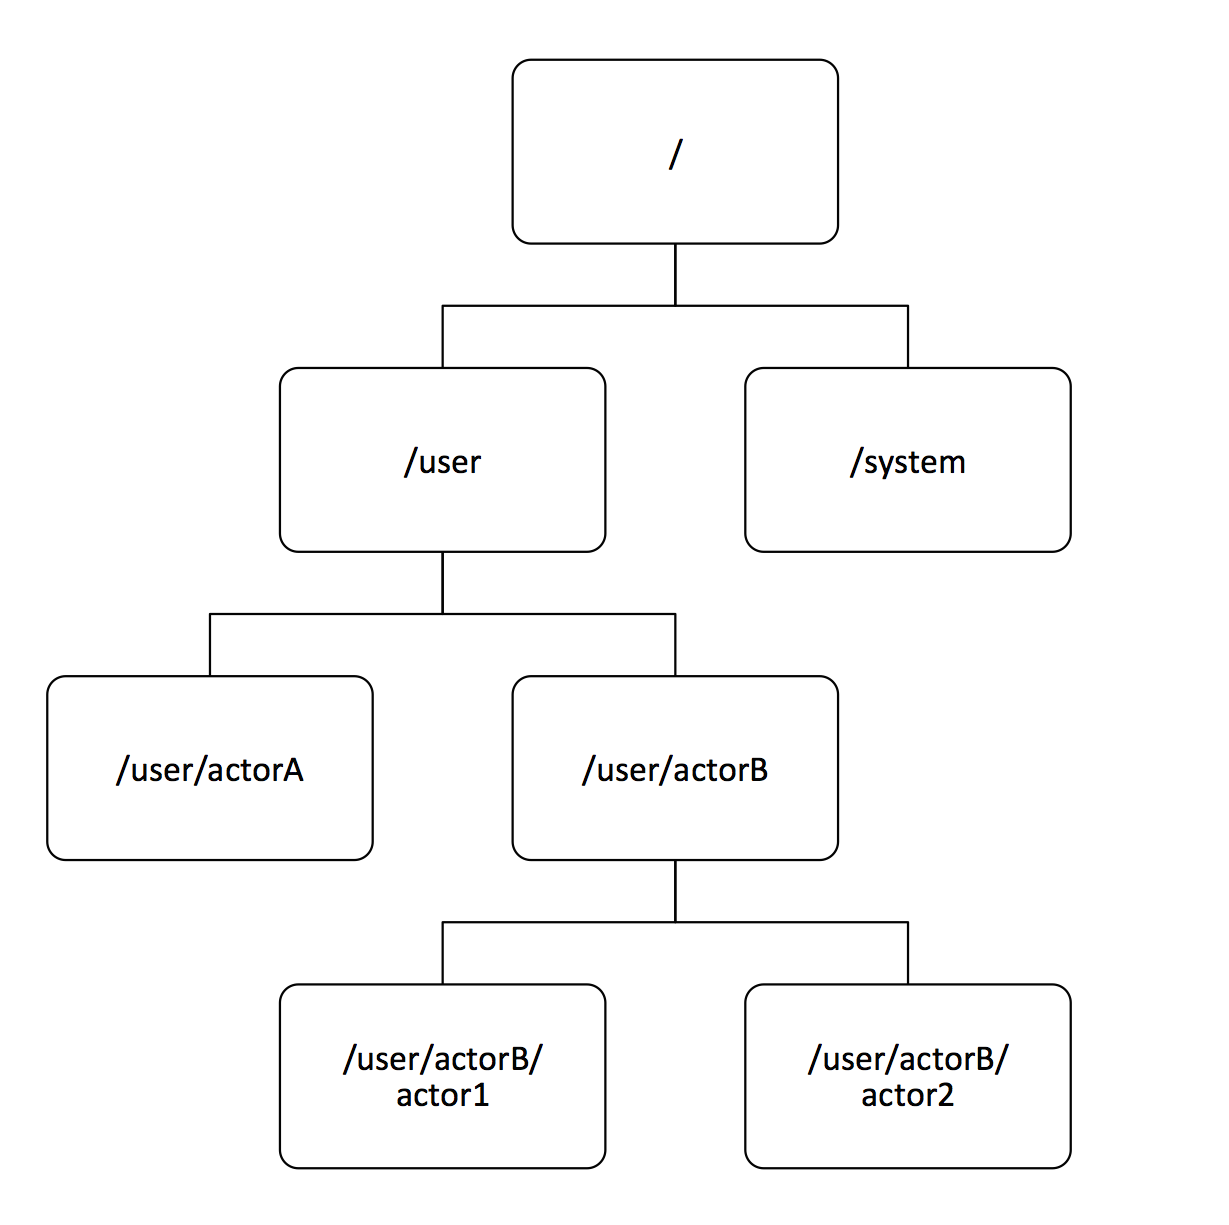
\includegraphics[scale=0.32]{figures/actorSystem}
  \caption[Hierarchy in actor system]{Hierarchy in actor system~\cite{akkaJavaDoc}}
  \label{fig:actorSystem}
\end{figure}

  \subsection{Message Passing in Akka}
  \label{subsec:akkaMessagePassing}
  In Akka, every actor has an event driven message inbox known as a ‘mailbox’. A mailbox buffers all incoming messages until they are processed. When a message is sent from one actor to another, the reference to the sender (an ActorRef) is automatically added to the message. Thus, during message processing a recipient actor has a reference to the sending actor through the \emph{sender} method~\cite{akkaJavaDoc}.

  Akka guarantees the order of direct message delivery between two actors. It is only applicable when the mailbox implementation in a receiver is a FIFO mailbox and the communication takes place only between the two actors without the involvement of intermediary actors. For instance, if an actor A1 sends messages M1, M2 and M3 to actor A2, the message M1 will be delivered before M2 and the message M2 before M3. If another actor A3 sends messages M4, M5 and M6 to A2 at the same time, the order of message delivery of M4, M5 and M6 will also be sequential. Nevertheless, there is no guarantee that the messages sent by A1 are delivered before the messages from A3, even if all of the messages from A1 were sent before A3 started sending messages~\cite{akkaJavaDoc}.

  The Akka Java documentation mentions rules for message sending: \cite{akkaJavaDoc}
  \begin{itemize}
    \item at-most-once delivery, i.e. no guaranteed delivery
    \item message ordering per sender–receiver pair
  \end{itemize}

‘At-most-once delivery’ means that a message is either not delivered at all (i.e. lost) or delivered only once. Thus, there is no duplicate delivery of a message.

  \subsection{Shared Mutable State}
  Since Akka runs on top of the JVM, there are pitfalls a programmer should know to avoid. Messages used to communicate between actors should be immutable. If messages are mutable and are mutated by an actor in the same JVM, bugs such as race conditions and even unpredictable behaviors might appear. Also, the sender method must not be closed over if the block of code could be run in another thread; for instance, replying to the sender actor inside a ‘Future’ block. In such cases, the sender reference must be captured into a local variable first, as the reference and behavior of the sender may change over time~\cite{akkaJavaDoc}.

  \subsection{Actor Supervision and Monitoring}
  \label{subsec:supervisionMonitoring}
  A supervising actor in Akka delegates tasks to its subordinates and monitors them for failure. When a child actor detects a failure, it suspends itself and its child actors and sends a message to its supervisor about the failure. According to Akka Java documentation\cite{akkaJavaDoc}, a supervisor may opt to perform one of four choices upon receiving a failure:
  \begin{enumerate}
    \item Resume the subordinate, keeping its accumulated internal state
    \item Restart the subordinate, clearing out its accumulated internal state
    \item Stop the subordinate permanently
    \item Escalate the failure, thereby failing itself
  \end{enumerate}

  When an actor is restarted by its supervising actor, the message that the actor was processing during the time of failure is lost and is not processed again. However, the messages that were in the mailbox remain safe and are processed after the restart~\cite{akkaJavaDoc}.

  \subsection{Routers}
  \label{subsec:akka-routers}
  Routers are specialized actors that act as a load balancer for the actors they supervise. Akka provides several built-in routing techniques:~\cite{akkaJavaDoc}
  \begin{itemize}
    \item Round Robin Router
    \item Random Router
    \item Smallest Mailbox Router
    \item Broadcast Router
    \item Scatter Gather First Completed Router
    \item Tail Chopping Router
    \item Consistent Hashing Router
  \end{itemize}

It is also possible to use a custom implementation of a router by extending the \emph{RoutingLogic} class from Akka's routing library.

  \subsection{Remote Actors in Akka}
  Actors in Akka are location transparent; they reside in a logical hierarchy of an actor system through which the physical location of an actor in the network can be determined. Location transparency allows Akka applications to be developed locally but deployed into distributed systems simply by changing configurations~\cite{akkaJavaDoc}.

  Peer-to-peer communication between actor systems is the basis for Akka Clustering. Akka's Documentation for Java~\cite{akkaJavaDoc} lists two design decisions for remoting:
\begin{enumerate}

  \item Communication between involved systems is symmetric: if system A can connect to system B then system B must also be able to connect to system A independently.

  \item The role of the communicating systems are symmetric in regards to connection patterns: there is no system that only accepts connections, and there is no system that only initiates connections.
\end{enumerate}

\autoref{lst:akkaRemoting} is taken from the website of Akka\footnote{\fullcite{akkaHome}} which is an example of configuration and code for deploying actors in remote nodes.

\begin{lstlisting}[caption=A sample Akka Configuration and Code for Remote Actors~\cite{akkaHome}, label=lst:akkaRemoting]
  // ------------------------------
  // config on all machines
  akka {
    actor {
      provider = akka.remote.RemoteActorRefProvider
      deployment {
        /greeter {
          remote = akka.tcp://MySystem@machine1:2552
        }
      }
    }
  }

  // ------------------------------
  // define the greeting actor and the greeting message
  public class Greeting implements Serializable {
    public final String who;
    public Greeting(String who) { this.who = who; }
  }

  public class GreetingActor extends UntypedActor {
    LoggingAdapter log = Logging.getLogger(getContext().system(), this);

    public void onReceive(Object message) throws Exception {
      if (message instanceof Greeting)
        log.info("Hello " + ((Greeting) message).who);
    }
  }

  // ------------------------------
  // on machine 1: empty system, target for deployment from machine 2
  ActorSystem system = ActorSystem.create("MySystem");

  // ------------------------------
  // on machine 2: Remote Deployment - deploying on machine1
  ActorSystem system = ActorSystem.create("MySystem");
  ActorRef greeter = system.actorOf(Props.create(GreetingActor.class), "greeter");

  // ------------------------------
  // on machine 3: Remote Lookup (logical home of "greeter" is machine2, remote deployment is transparent)
  ActorSystem system = ActorSystem.create("MySystem");
  ActorSelection greeter = system.actorSelection("akka.tcp://MySystem@machine2:2552/user/greeter");
  greeter.tell(new Greeting("Sonny Rollins"), ActorRef.noSender());
\end{lstlisting}

  \subsection{Clustering in Akka}
  Akka does not have a central server. Instead, it uses a peer-to-peer based gossip protocol to form a cluster. Thus, there is no single point of failure or single point of bottleneck in the system. Adding a new member in a distributed system requires significant amount of time because of the nature of the gossip protocol. In a benchmark~\cite{akkaBenchmark} performed by Patrik Nordwall\footnote{Patrick Nordwall is a developer of Akka at Typesafe Inc.}, adding a node to a cluster of at least 1500 nodes took around 15 to 20 seconds on average.


\section{The Dart Language}
\label{sec:dart}
  \subsection{Overview}
  Dart is an open-source, class-based, single-inheritance, pure object-oriented programming language developed by Google~\cite{dartEcma}. The Dart language is inspired by Smalltalk, Strongtalk, Erlang, C\# and JavaScript~\cite{sethladd}.

  Dart code is not compiled before running; it is read and executed directly from source code by the Dart Virtual Machine (VM). Dart provides a homogeneous system that encompass both client as well as server as the Dart VM can be embedded in browsers. A version of Chromium – ‘Dartium’ already has a Dart VM built into it~\cite{sethladd}.

  Programs in Dart are optionally typed. They can be executed in two modes, checked mode and production mode. In checked mode incorrect static type annotations produce compile time errors. Whereas, in production mode type annotations are completely ignored~\cite{dartEcma}.

  Furthermore, Dart allows developers to code in a uniform way for both server as well as client since the Dart Virtual Machine (VM) can be embedded in browsers.

  Dart has an automatic garbage collection system, which means the memory occupied by objects which are not in use and which have no references are reclaimed periodically.
  %
  % Developers of Dart believe that JavaScript has been pushed to its limit and the web apps developed in JavaScript are far too slow even though JavaScript engines are fast. They claim Dart offers a better solution to build larger and more complex web applications\cite{laddWalrath}.

Some of its important features and advantages are:
  \begin{itemize}
    \item Easy to learn syntax
    \item Dart supports types, but they are optional
    \item Scales from small scripts to large and complex applications
    \item Supports safe concurrency with isolates
    \item Supports code sharing
    \item Translates to JavaScript so that code can be run in web-browsers that do not have the Dart VM yet
    \item Unified development for client and server
    \item Runs in client as well as on server
    \item Has been gaining popularity and adoption in recent years
\end{itemize}

  \subsection{Dart and JavaScript}
  Code written in Dart can be translated to JavaScript using a tool – ‘dart2js’. ‘Dart2js’ is bundled with the Dart SDK (Software Development Kit). As popular web browsers like Mozilla Firefox, Google Chrome and Safari do not have a Dart Virtual Machine embedded, the ability to translate source code from Dart to JavaScript lets Dart programs run in any modern browser without needing to manually port the source code to JavaScript.

  \subsection{Asynchronous Programming in Dart}
  Most programming languages use callback functions for asynchronous programming. Dart provides some additional alternatives along with callback functions \textendash~Future and Stream objects. A ‘Future’ is a promise for a result which will be returned after an arbitrary amount of time. A ‘Stream’ is a way to get a sequence of values, such as events or data from ports.

  \subsection{Isolates}
  \label{sec:isolates}
  Although Dart programs are single threaded, concurrency is supported using actor-like entities called isolates. An isolate has its own memory and own thread of control. Message passing is the sole way to communicate between isolates. No state is ever shared between isolates~\cite{dartEcma}.

  An isolate has its own heap memory different from the main isolate (the top level isolate). It is possible for a child isolate to throw exceptions and errors, for example when exhausting its memory. If exceptions are not handled properly, it forces the isolate to be shutdown.

  In Dart, when an isolate is spawned, usually a ‘sending port’ is sent as the initial message (by the spawner), so that the spawner and “spawnee” can communicate with each other. The “spawnee” uses the sending port sent by the spawner to reply.

  An isolate can spawn another isolate which can further spawn isolates and have control over them. Thus, the spawner can supervise the “spawnee”. The spawner can pause the “spawnee” or terminate it~\cite{dartApiIsolate}~\footnote{Pausing and terminating an isolate is not available in Dart 1.7.2 or older versions}.

  Modern web browsers run on multi-core CPUs, even on mobile platforms. To take advantage of multiple cores, developers traditionally use shared-memory threads running concurrently. However, shared-state concurrency is error prone and can lead to complicated code. Thus, instead of threads, all Dart code runs inside of isolates. Each isolate has its own memory heap, ensuring that no isolate’s state is accessible from any other isolate~\parencite{laddWalrath}.

  \subsubsection{Spawning an Isolate}
    There are two ways to spawn an isolate: using \emph{Isolate.spawnUri()} or using \emph{Isolate.spawn()}. \emph{Isolate.spawn()} uses a top level function of an isolate to spawn that isolate. The top level function may reside in the same class or may belong to another class. \emph{Isolate.spawnUri()} spawns an isolate using the source code of a file from a given location. The location can be a remote http/https \acrshort{uri} or a path to a source file in the local disk. To spawn an isolate using \emph{Isolate.spawnUri()}, the source file must have an entry point function named \emph{main()}.
    The newly spawned isolate shares the same code as the spawner isolate~\cite{dartApiIsolate}.

  \subsubsection{Communication Between Two Isolates}
  After an isolate is spawned, it is recommended to send its SendPort to the spawner isolate so that the “spawner” and “spawnee” can communicate via message passing. SendPort and ReceivePort are used by the isolates to communicate with each other.

  The example in \autoref{lst:isolateSample} shows how an isolate is spawned using \emph{spawnUri()} and how to perform basic communications between two isolates in Dart. As shown in this example, the message sending is performed after the SendPorts are exchanged between the isolates.

\begin{lstlisting}[caption=A simple example of isolate communication in dart, label=lst:isolateSample]

  //sample.dart
  import 'dart:isolate';

  main(var args, SendPort sendPort) {
    ReceivePort receivePort = new ReceivePort();
    SendPort sendport;
    sendPort.send(receivePort.sendPort);

    receivePort.listen((var message) {
      if(message is SendPort) {
        sendPort = message;
      } else if(message is String) {
        print("Received: $message");
      } else {
        sendPort.send("Unknown Message");
      }
    });
  }

  //app.dart
  import 'dart:isolate';

  main() {
    ReceivePort receivePort = new ReceivePort();
    SendPort sendPort;  Isolate.spawnUri(Uri.parse("sample.dart"),null,receivePort.sendPort); // Spawns an isolate from sample.dart file

    receivePort.listen((var message) {
      if(message is SendPort){
        sendPort = message;
        sendPort.send(receivePort.sendPort);
        sendPort.send("Hello");
        sendPort.send(["a", "list", "datatype"]);
      } else if(message is String) {
        print("Reply: $message");
      }
    });
  }
\end{lstlisting}

  \subsubsection{Difference from Actors}
  Although Dart isolates do not have shared state and use message-passing as the only means of communication between two isolates, isolates differ from actors~[\autoref{sec:actorProgramming}] in many ways. The most significant difference is the principle behind spawning of an actor and spawning of an isolate. An actor should be very lightweight and cheap to spawn, but Dart isolates are resource heavy and slow to spawn. The implementation of actors found in languages like Erlang~[\autoref{sec:erlang}] and the Akka toolkit~[\autoref{sec:akka}] can be considered much closer to Hewitt's actor model.

  The number of actors that can be spawned per GigaByte of heap memory in Akka reaches up to 2.7 million~\cite{akkaHome}. A simple isolate in Dart consumes 5 to 7 MegaBytes\footnote{Based on the memory consumption of the two isolates from \autoref{lst:isolateSample}} of memory, so the number of isolates per GigaByte of heap only reaches a few hundred. Based on these observations, it would be appropriate to say that the current\footnote{Dart version 1.7.2} implementation of an isolate in Dart is \textemdash{} similar to a thread with properties like an actor.

  \subsubsection{Limitations of Isolates}
  Although Dart isolates follow the asynchronous message passing model which is suitable for distributed systems, it is not possible for an isolate in one Dart VM to send message to an isolate in another Dart VM. A message exchange between two isolates via SendPort/ReceivePort is possible only if the isolates are spawned locally in the same Dart virtual machine. This is a hindrance in making isolates distributed.

\section{RabbitMQ - A Message Broker System}
\label{sec:rabbitmq}
  RabbitMQ is an open-source simple message broker software that implements the Advanced Message Queuing Protocol (AMQP). It serves as an intermediary for message passing between applications or components. It give applications a common platform to send and receive messages, and keeps the messages safe until intended subscribers receive them~\cite{rabbitmqFeatures}.

  Messaging enables software applications to connect and scale. Applications can connect to each other as components of a larger application, or to user devices and data. Messaging is asynchronous, decoupling applications by separating sending and receiving data. In RabbitMQ, messages are routed through exchanges before arriving at queues. RabbitMQ features several built-in exchange types for typical routing logic~\cite{rabbitmqFeatures}.

  RabbitMQ allows several servers of a local network to form a cluster. The cluster forms a single logical broker and queues are mirrored across several machines, which means applications that use it may connect to any of the servers that belong to the cluster~\cite{rabbitmqFeatures}.

RabbitMQ supports several protocols for enqueuing and dequeuing messages:
\begin{itemize}
  \item AMQP (Several versions)\\
  The Advanced Message Queuing Protocol (AMQP) was designed to provide reliability and interoperability. It provides messaging, including reliable queuing, topic-based publish-and-subscribe messaging, flexible routing, transactions, and security. AMQP exchanges route messages based on topic and headers~\cite{andyPiperVmware}.
  Despite the fact that there are many different language implementations\footnote{Python, Java, Ruby, PHP, C\#, Erlang etc.~\cite{rabbitmqGetstarted}} and examples for using AMQP in RabbitMQ, it is still not available for the Dart language.

  \item STOMP\\
  STOMP~[\autoref{sec:stomp}] is a text-based messaging protocol emphasizing simplicity. More about STOMP is discussed in \autoref{sec:stomp}.

  RabbitMQ supports STOMP via a plugin \textendash{} ‘rabbitmq\textunderscore{}stomp’.

  \item MQTT\\
  Message Queue Telemetry Transport was developed by IBM. It provides lightweight publish-and-subscribe messaging, targeted for devices with limited resources and network bandwidth. Hence, the design principles and aims of MQTT are simpler and more focused than those of AMQP~\cite{andyPiperVmware}.

  RabbitMQ supports MQTT 3.1 via a plugin.
  \item HTTP\\
  HTTP is not a messaging protocol. Nevertheless, with the help of the listed technologies that use HTTP as their sub protocol, RabbitMQ can transmit messages over HTTP~\cite{rabbitmqProtocols}.

  \begin{description}
    \item{Management Plugin}\\
    It supports a simple HTTP API to send and receive messages. This is primarily intended for diagnostic purposes but can be used for low volume messaging without reliable delivery.
    \item{Web-STOMP Plugin}\\
    The plugin supports STOMP messaging to the browser using WebSockets. For older browsers that do not have support for WebSockets, fallback mechanisms provided by SockJS\footnote{SockJS is a JavaScript library that emulates WebSocket in browsers} are used.
    \item{JSON-RPC channel Plugin}\\
    This plugin supports AMQP 0-9-1 messaging over JSON-RPC\footnote{JSON-RPC is JSON encoded Remote Procedure Call protocol}. It is a synchronous protocol, thus the asynchronous delivery property of AMQP is emulated by polling.
  \end{description}
\end{itemize}

  \subsection{Message Queues in RabbitMQ}
  In RabbitMQ, a queue is a mailbox name where  messages are stored. It can buffer a large quantity of messages bounded only by the available resources of the machine.

  RabbitMQ receives messages from a client via one of the protocols described in [\autoref{sec:rabbitmq}]. When sending a message, the client specifies the name of the queue where the message should be enqueued. Meanwhile, the subscribing client of the queue receives a message either as soon as the message is available in the queue, or when the client sends a request for dequeue, or only after acknowledging a previously dequeued message. This depends upon the parameters used during subscription to the queue.

  If inflow of messages in a queue is faster than the outflow of the messages to its subscribers, both enqueuing as well as dequeuing becomes slower. Since messages are buffered into memory, as the quantity of messages increases the consumption of memory also increases. If there is a sudden increase in the inflow of messages, the incoming messages take more CPU time which results in the overall decrease of outflow of messages to consumers~\cite{sizingYourRabbits}.

  \subsection{RabbitMQ and Prefetch-count}
  \label{subsec:rabbitmqPrefetch}
  The prefetch-count Quality of Service (QoS) setting in RabbitMQ by default is set to unlimited. Which means RabbitMQ empties the queue as fast as possible to consumers. Setting the prefetch-count to unlimited might result in ‘out of memory’ or ‘stack overflow’ errors in the consumers. Again, setting the prefetch-count too low can hamper the performance of the whole application while setting it too high can cause  ‘out of memory’ exceptions. Hence, based on the requirement and design of the consumer application, an appropriate prefetch-count should be determined.

  \autoref{fig:rabbitmqBenchmark} is the result of a benchmark\footnote{posted by Simon MacMullen on April 25th, 2012 at 2:47 pm} that shows how the throughput of a queue varies when prefetch count is changed for different numbers of consumers.
\begin{figure}[H]
  \centering
  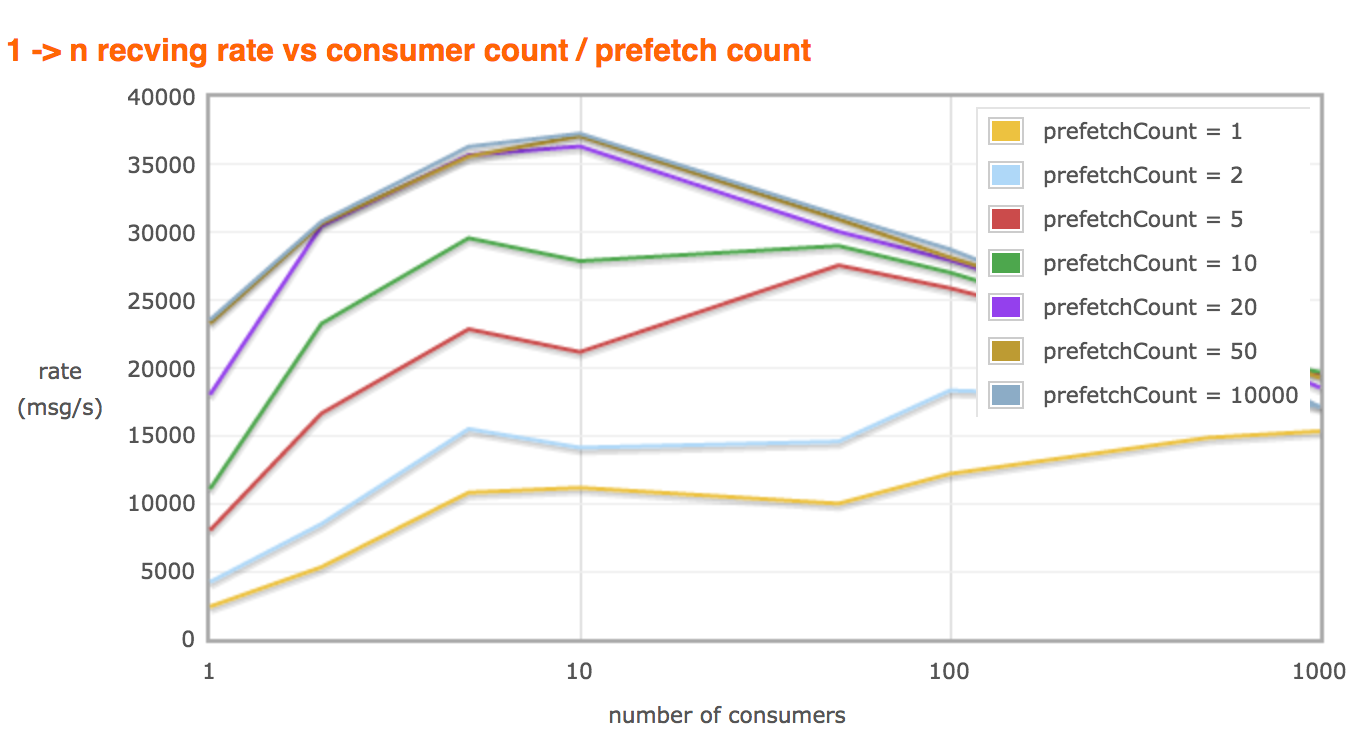
\includegraphics[width=1\textwidth]{figures/rabbitmqPrefetch}
  \caption[Chart showing performance variation when prefetch count is changed in the consumer]{Chart\footnotemark showing performance variation when prefetch count is changed in the consumer}
  \label{fig:rabbitmqBenchmark}
\end{figure}
\footnotetext{Source: \fullcite{rabbitmqPerformance}}

\section{STOMP}
\label{sec:stomp}
  STOMP stands for Simple (or Streaming) Text Orientated Messaging Protocol. It is an alternative to other open messaging protocols such as AMQP. STOMP provides an interoperable format for clients to communicate with a message broker system that supports STOMP. It provides interoperability for different languages, platforms and brokers~\cite{stomp}.
  STOMP is designed to be a lightweight protocol that is easy to implement in both client and server.
  \subsection{Protocol Overview}
  STOMP is a frame-based protocol. A frame consists of a command, a set of optional headers and an optional body. STOMP is text based but it allows the transmission of binary messages as well~\cite{stomp}. A STOMP client can either be a producer or consumer.
  % As a producer a message can be sent to a destination server using SEND frame. Meanwhile, as a consumer, SUBSCRIBE frame should be sent for subscription of a message for a given destination. Then, the messages are received as MESSAGE frames.

  \subsection{STOMP Library for Dart}
  \label{subsec:stompForDart}
  Dart's ‘pub’\footnote{http://pub.dartlang.org} is a public library sharing platform which allows users to share and reuse Dart code.

  Given that Dart is a fairly new language, there is no AMQP client for RabbitMQ yet. As mentioned above in section~\ref{sec:rabbitmq} RabbitMQ also supports STOMP. An open source STOMP client\footnote{https://github.com/rikulo/stomp} in Dart is available in Dart's ‘pub’ created by the ‘Potix corporation’. It can perform most of the basic operations with a message broker system like connecting, creating queues, subscribing, enqueuing and dequeuing.


\section{WebSockets}
\label{sec:websocket}
  The WebSocket protocol enables two-way communication between client and server over a single TCP connection. It uses an origin-based security model, which is found in web browsers. It can be used for a variety of web applications: games, stock tickers, multiuser applications, user interfaces exposing server-side services in real time, etc~\cite{rfc6455}.

  Since HTTP was not initially designed for bidirectional communication, the WebSocket Protocol is designed to displace other existing bidirectional communication technologies that are based on HTTP~\cite{rfc6455}.

  WebSockets use two URI schemes: “ws://” for normal WebSocket connections and “wss://” for secured WebSocket connections~\cite{rfc6455}.

\subsection{Security}
  The WebSocket protocol uses the origin model to restrict which web pages can contact a WebSocket server when the WebSocket protocol is used from a web page~\cite{rfc6455}.

   A WebSocket server reads the handshake sent by a client to establish a connection. Thus, an attempt to connect to a WebSocket from other protocols cannot succeed if it is not made by a WebSocket client~\cite{rfc6455}.

\subsection{Establishing a Connection}
  When establishing a WebSocket connection, an HTTP server receives a regular GET request with an offer to upgrade to a WebSocket. The server responds to the request to complete the handshake and establish the connection. Then the communication takes place in full-duplex mode~\cite{rfc6455}.
